% =============================================================================
% FIGURE PLACEHOLDER - Global CSO Map
% =============================================================================
% This is a placeholder for the actual map figure
% Replace with \includegraphics command and subcaption environments when ready

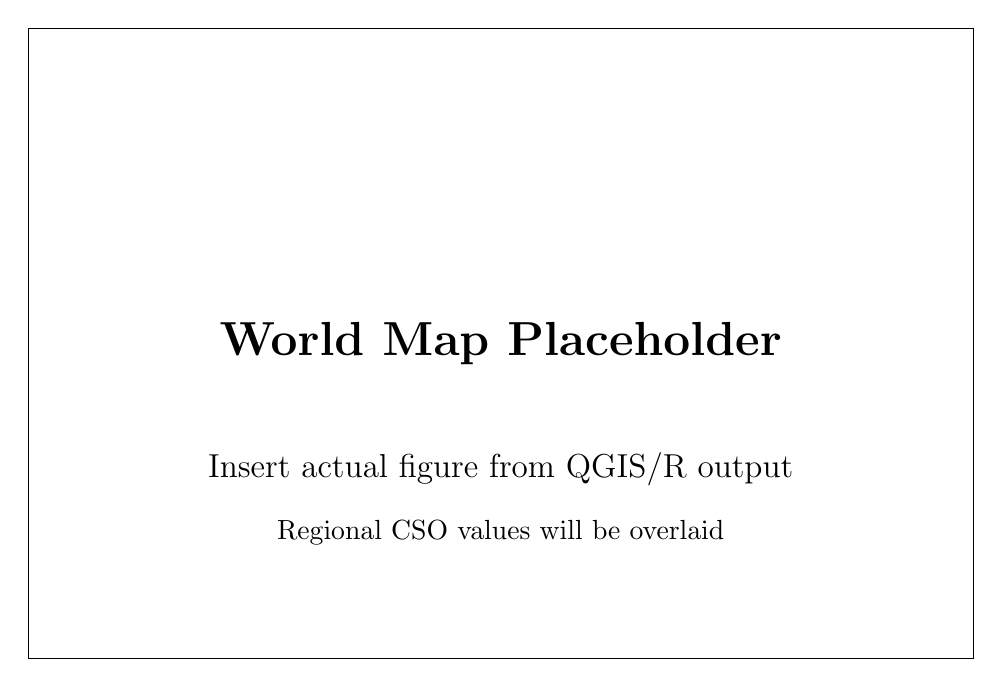
\begin{tikzpicture}[scale=0.8]
    % World map placeholder with regional boxes
    \draw (0,0) rectangle (15,10);
    \node at (7.5,5) {\LARGE\bfseries World Map Placeholder};
    \node at (7.5,3) {\large Insert actual figure from QGIS/R output};
    \node at (7.5,2) {Regional CSO values will be overlaid};
\end{tikzpicture}

%\begin{figure}[htbp]
%    \centering
%    \begin{tikzpicture}[scale=0.9, transform shape]
%        \draw[fill=green!30] (0,0) rectangle (3,2) node[midway] {AFRO};
%        \draw[fill=blue!30] (3,0) rectangle (6,2) node[midway] {AMRO};
%        \draw[fill=yellow!30] (6,0) rectangle (9,2) node[midway] {EMRO};
%        \draw[fill=red!30] (9,0) rectangle (12,2) node[midway] {EURO};
%        \draw[fill=purple!30] (0,-2) rectangle (4,-4) node[midway] {SEARO};
%        \draw[fill=orange!30] (4,-2) rectangle (12,-4) node[midway] {WPRO};
%
%        % Legend
%        \node[draw, fill=green!30] at (1,-5) {CSO > 0.7};
%        \node[draw, fill=yellow!30] at (4,-5) {0.3 < CSO < 0.7};
%        \node[draw, fill=red!30] at (8,-5) {CSO < 0.3};
%    \end{tikzpicture}
%    \caption[Global CSO distribution by WHO region]{Geographic distribution
%    of capsid sequence observability (CSO) scores across WHO regions.
%    Green indicates adequate surveillance capacity (CSO > 0.7);
%    yellow indicates moderate capacity (0.3--0.7); red indicates
%    critical gaps (CSO < 0.3).}
%\end{figure}